\documentclass{article}

\usepackage{graphicx}
\usepackage{tikz}
\usepackage{tikzsymbols}
\usetikzlibrary{calc,patterns,shapes.geometric}
\pagestyle{empty}
\usepackage[margin=0pt]{geometry}
\geometry{papersize={14in,12in}}

\def\centerarc[#1](#2)(#3:#4:#5){\draw[#1] ($(#2)+({#5*cos(#3)},{#5*sin(#3)})$) arc (#3:#4:#5);}

\begin{document}
	\begin{figure}
		\centering
		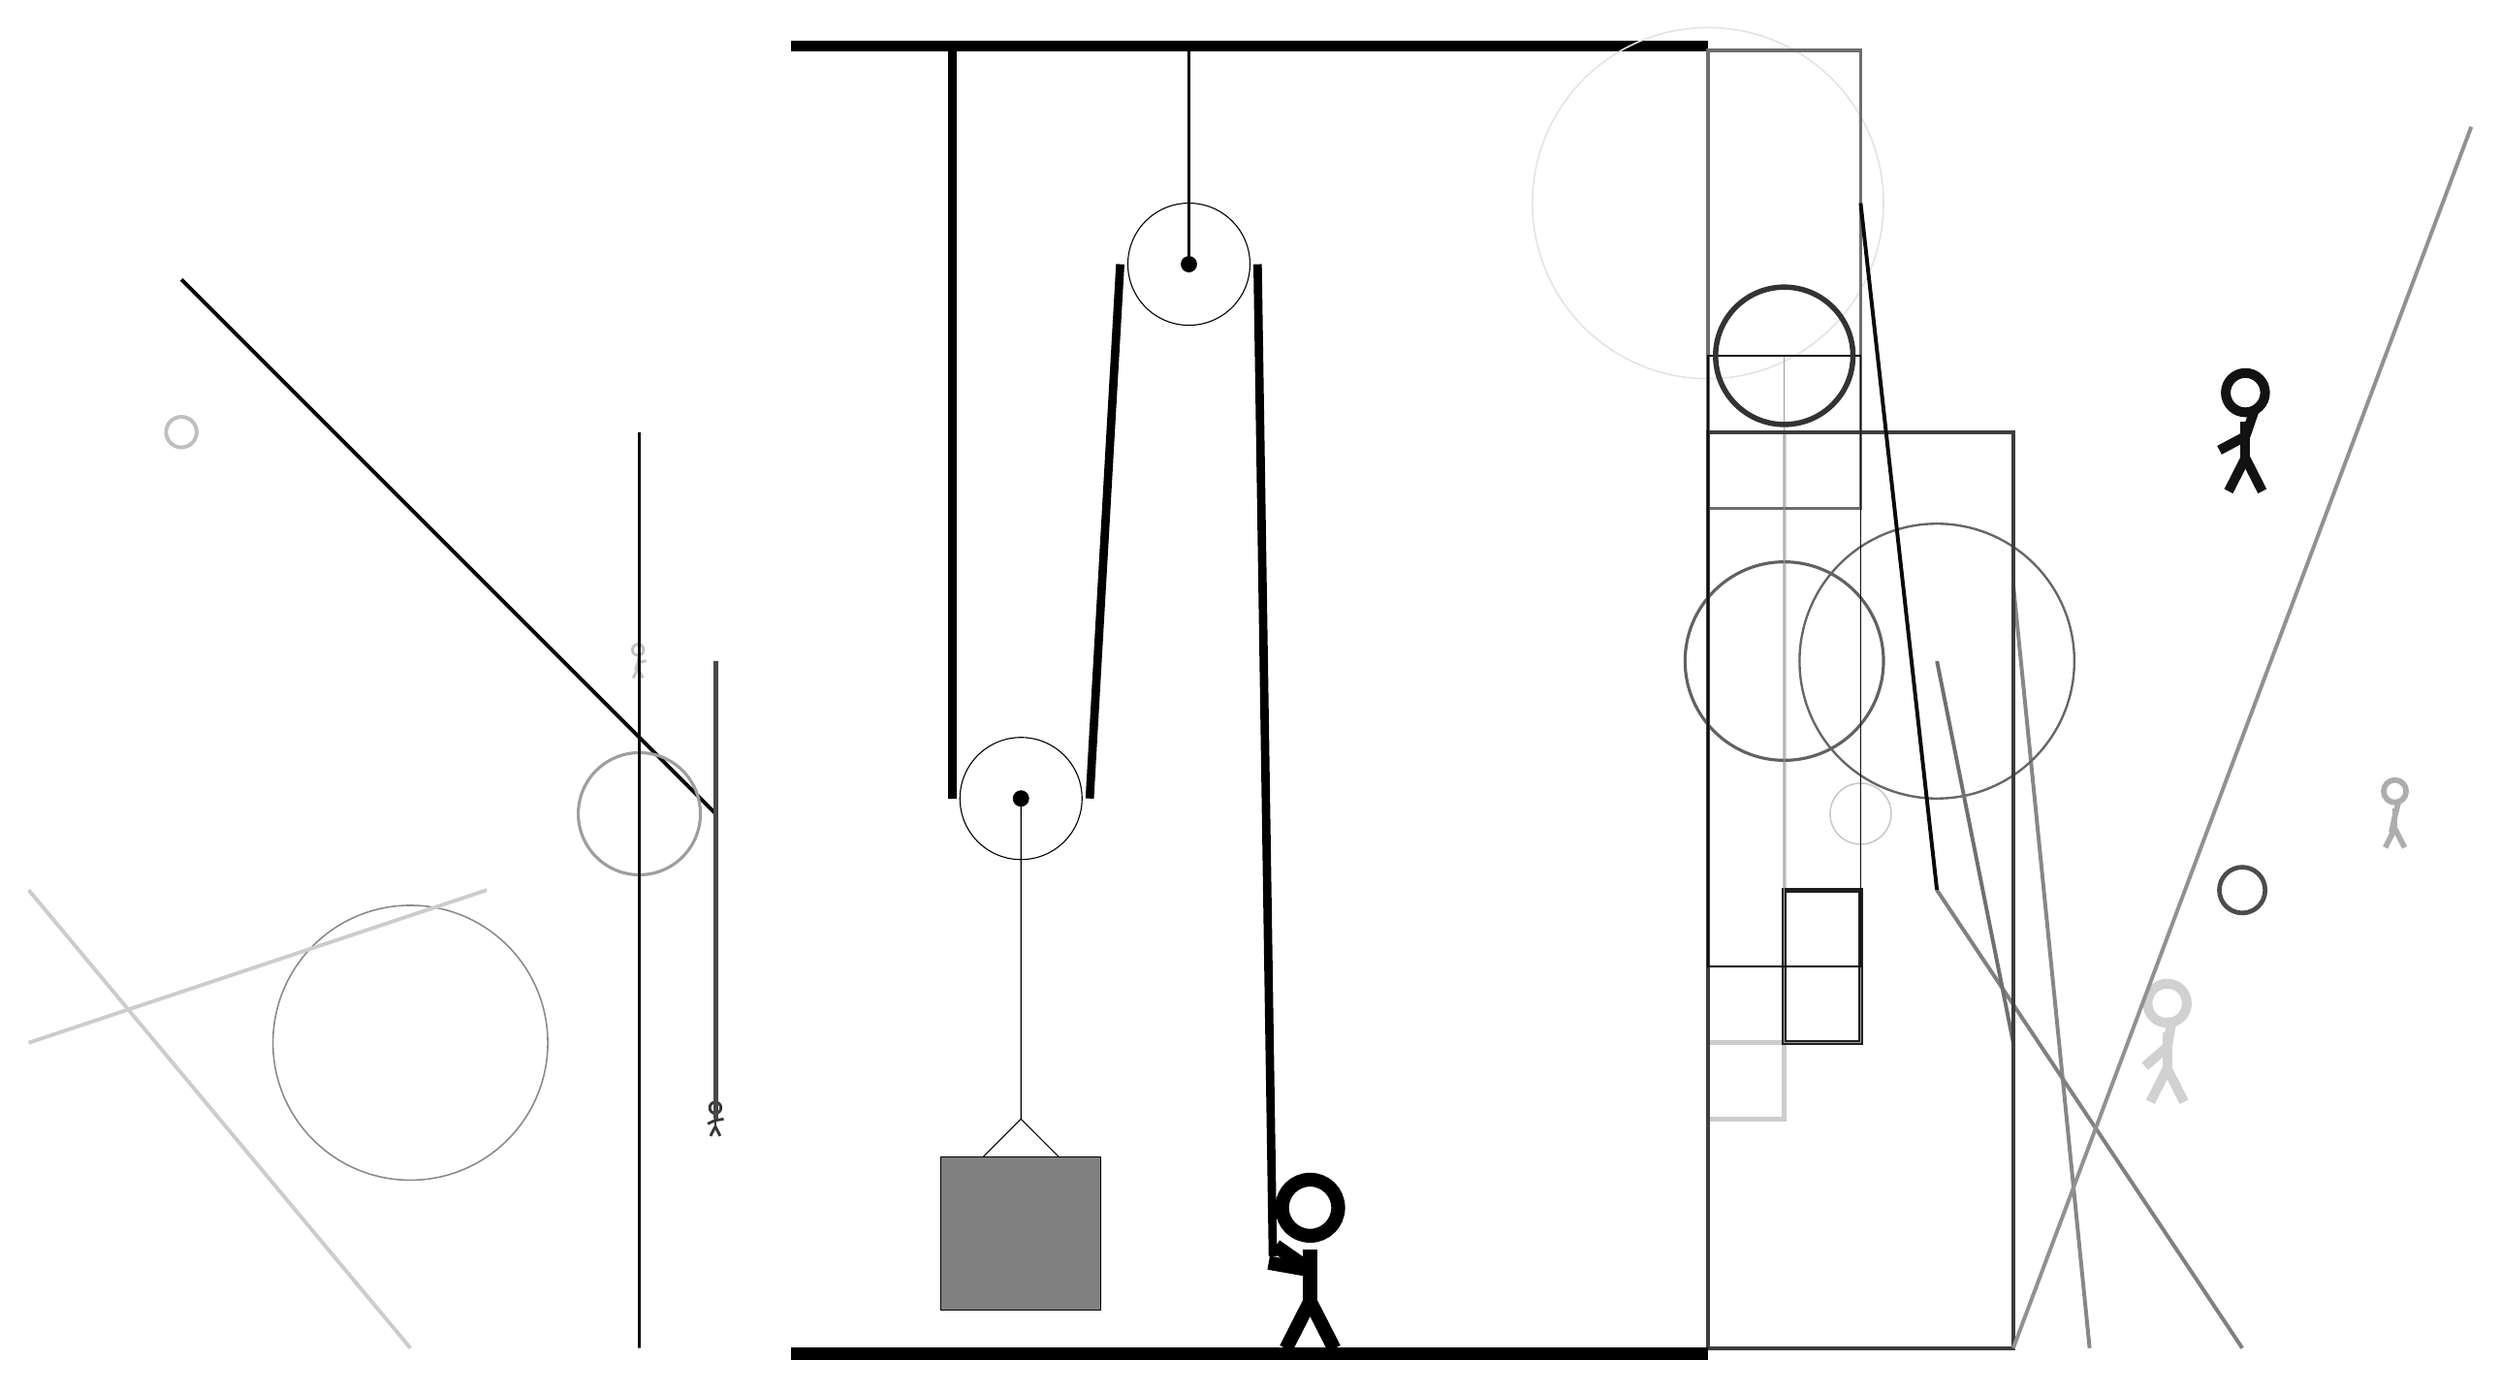
\begin{tikzpicture}
			%%%%% START %%%%%
			
			\draw[fill=black] (-2, 14) rectangle (10, 14.125);
			
			\draw (3.2, 11.2) circle (0.8);
			\draw[fill=black] (3.2, 11.2) circle (0.1);
			\draw[thick] (3.2, 11.2) -- (3.2, 14);
			
			\draw (1, 4.2) circle (0.8);
			\draw[fill=black] (1, 4.2) circle (0.1);
			
			\draw (1, 4.2) -- (1, 0) -- (0.5, -0.5);
			\draw (1, 0) -- (1.5, -0.5);
			\draw[fill=black!50] (-0.05, -0.5) rectangle (2.05, -2.5);
			
			\draw [line width=0.2mm, color=black!21](12, 4) circle (0.4);
			
			\draw[line width=0.7mm, color=black!41] (12, 14) rectangle (12, 14);
			\draw[line width=0.5mm, color=black!97](-3, 4) -- (-10, 11);
			\draw [line width=0.6mm, color=black!70](17, 3) circle (0.3);
			\draw[line width=0.5mm, color=black!19] (10, 0) rectangle (11, 9);
			
			\draw [line width=0.2mm, color=black!46](-7, 1) circle (1.8);
			\node[line width=0.4mm, color=black!79] at (-3, 0) {\Strichmaxerl[2][25][8]};
			\draw[line width=0.6mm, color=black!20] (11, 1) rectangle (10, 0);
			\draw [line width=0.2mm, color=black!11](10, 12) circle (2.3);
			\draw [line width=0.4mm, color=black!62](11, 6) circle (1.3);
			\draw[line width=0.5mm, color=black!47](14, 7) -- (15, -3);
			
			\draw[line width=0.5mm, color=black!20](-6, 3) -- (-12, 1);
			\node[line width=0.6mm, color=black!24] at (-4, 6) {\Strichmaxerl[2][71][10]};
			
			\draw [line width=0.5mm, color=black!81](16, 11) circle (0.0);
			\draw[line width=0.5mm, color=black!50](13, 3) -- (17, -3);
			\draw [line width=0.3mm, color=black!60](13, 6) circle (1.8);
			
			\draw[line width=0.5mm, color=black!56](13, 6) -- (14, 1);
			\draw [line width=0.4mm, color=black!38](-4, 4) circle (0.8);
			\draw[line width=0.7mm, color=black!72] (-3, 0) rectangle (-3, 6);
			\draw[line width=0.5mm, color=black!20](-7, -3) -- (-12, 3);
			\draw[line width=0.4mm, color=black!57] (10, 14) rectangle (12, 8);
			
			\draw[line width=0.6mm, color=black!88] (12, 1) rectangle (11, 3);
			\draw [line width=0.5mm, color=black!25](-10, 9) circle (0.2);
			\node[line width=0.2mm, color=black!93] at (17, 9) {\Strichmaxerl[7][28][71]};
			\draw[line width=0.3mm, color=black!95] (-4, 9) rectangle (-4, -3);
			
			\draw[line width=0.2mm, color=black!38] (12, 10) rectangle (11, 1);
			\draw[line width=0.5mm, color=black!76] (10, 9) rectangle (14, -3);
			\draw[line width=0.5mm, color=black!96](13, 3) -- (12, 12);
			
			\draw[line width=0.2mm, color=black!94] (12, 10) rectangle (10, 2);
			\node[line width=0.7mm, color=black!32] at (19, 4) {\Strichmaxerl[4][78][76]};
			\node[line width=0.4mm, color=black!18] at (16, 1) {\Strichmaxerl[7][41][80]};
			
			\draw[line width=0.5mm, color=black!43](14, -3) -- (20, 13);
			\draw [line width=0.7mm, color=black!80](11, 10) circle (0.9);
			
			
			\draw[line width=1.1mm] (0.1, 14) -- (0.1, 4.2);
			\centerarc[line width=1.1mm](1, 4.2)(180:360:0.9);
			\draw[line width=1.1mm](1.9, 4.2) -- (2.3, 11.2);
			\centerarc[line width=1.1mm](3.2, 11.2)(0:180:0.9);
			\draw[line width=1.1mm](4.1, 11.2) -- (4.3, -1.8);
			
			\node at (4.7, -1.9) {\Strichmaxerl[10][-35][170]};
			
			\draw[fill=black] (-2, -3) rectangle (10, -3.15);
			
			%%%%% END %%%%%
		\end{tikzpicture}
	\end{figure}	
\end{document}